\iffalse
\let\negmedspace\undefined
\let\negthickspace\undefined
\documentclass[journal,12pt,twocolumn]{IEEEtran}
\usepackage{cite}
\usepackage{amsmath,amssymb,amsfonts,amsthm}
\usepackage{algorithmic}
\usepackage{graphicx}
\usepackage{textcomp}
\usepackage{xcolor}
\usepackage{txfonts}
\usepackage{listings}
\usepackage{enumitem}
\usepackage{mathtools}
\usepackage{gensymb}
\usepackage{comment}
\usepackage[breaklinks=true]{hyperref}
\usepackage{tkz-euclide} 
\usepackage{listings}
\usepackage{gvv}                                        
\def\inputGnumericTable{}                                 
\usepackage[latin1]{inputenc}                                
\usepackage{color}                                            
\usepackage{array}                                            
\usepackage{longtable}                                       
\usepackage{calc}                                             
\usepackage{multirow}                                         
\usepackage{hhline}                                           
\usepackage{ifthen}                                           
\usepackage{lscape}
\newtheorem{theorem}{Theorem}[section]
\newtheorem{problem}{Problem}
\newtheorem{proposition}{Proposition}[section]
\newtheorem{lemma}{Lemma}[section]
\newtheorem{corollary}[theorem]{Corollary}
\newtheorem{example}{Example}[section]
\newtheorem{definition}[problem]{Definition}
\newcommand{\BEQA}{\begin{eqnarray}}
\newcommand{\EEQA}{\end{eqnarray}}
\newcommand{\define}{\stackrel{\triangle}{=}}
\theoremstyle{remark}
\newtheorem{rem}{Remark}
\begin{document}

\bibliographystyle{IEEEtran}
\vspace{3cm}

\title{GATE: CH - 58.2022}
\author{EE23BTECH11224 - Sri Krishna Prabhas Yadla$^{*}$% <-this % stops a space
}
\maketitle
\newpage
\bigskip

\renewcommand{\thefigure}{\arabic{figure}}
\renewcommand{\thetable}{\arabic{table}}


\vspace{3cm}
\textbf{Question:} In the block diagram shown in the figure, the transfer function $G=\frac{K}{\tau s+1}$ with $K>0$ and $\tau>0$. The maximum value of $K$ below which the system remains stable is \rule{1cm}{0.15mm}(rounded off to two decimal places) \hfill (GATE CH 2022)
\begin{figure}[htbp]
	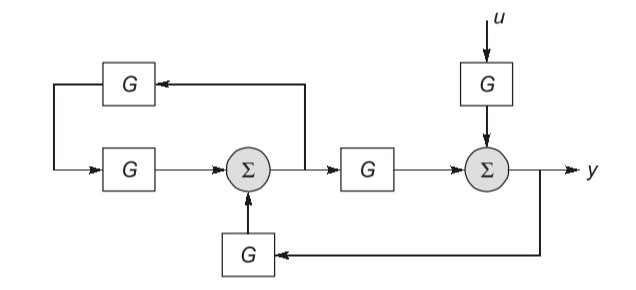
\includegraphics[width=\columnwidth]{2022/CH/58/figs/question.jpg}
	\label{fig:question}
\end{figure}\\
\solution
\fi
\begin{table}[htbp]
	\centering
	\def\arraystretch{1.5}
	\begin{tabular}{|c|c|c|}
\hline
Parameter & Value & Description \\
\hline 
G & $\frac{K}{\tau s+1}$ &Transfer function shown in blocks\\
\hline
Y & &Laplace transform of y(output)\\
\hline
U & &Laplace transform of u(input)\\
\hline
X,Z & &Laplace transform of x and z\\
\hline
T & $\frac{Y}{U}$ &Transfer function of complete system \\
\hline
\end{tabular}

	\caption{Parameters}
	\label{tab:parameters}
\end{table}
\begin{figure}[htbp]
	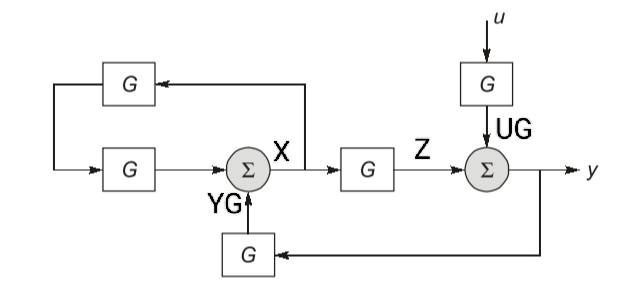
\includegraphics[width=\columnwidth]{2022/CH/58/figs/fig1.jpg}
	\caption{Block Diagram}
	\label{fig1}
\end{figure}
\begin{align}
X &= XG^2+YG \\
\implies X &= \frac{YG}{1-G^2}\\
Z &= XG\\
Y &= Z+UG\\
Y &= XG+UG\\
Y &= \frac{YG^2}{1-G^2}+UG\\
\implies Y &= \frac{UG(1-G^2)}{1-2G^2} 
\end{align}
From \tabref{tab:parameters},
\begin{align}
T &= \frac{G(1-G^2)}{1-2G^2}\\
&= \frac{K\brak{1-\frac{K^2}{(\tau s+1)^2}}}{\brak{1-\frac{2K^2}{(\tau s+1)^2}}(\tau s+1)}\\
&= \frac{K(\tau^2s^2+2\tau s+1-K^2)}{\tau^3s^3+3\tau^2s^2+(3\tau-2K^2\tau) s+1-2K^2}
\end{align}
% Here the denominator of G is \tau s + 1. Since \tau>0, 1/(\tau s+1) will have ROC: Re(s)>-1/\tau which will contain imaginary axis so it can be neglected here as we want for stability.
So, Characteristic equation : $1-2G^2 = 0$ 
\begin{align}
1-2\frac{K^2}{(\tau s+1)^2}&= 0 \\
\implies \tau^2s^2+2\tau s+1-2K^2 &= 0
\end{align}
For a characteristic equation $a_0s^n+a_1s^{n-1}+a_2s^{n-2}+...a_n=0$,
\begin{table}[htbp]
\setlength{\extrarowheight}{8pt}
\centering
\begin{tabular}{|c|c|c|c|c|}
\hline 
$s^n$ & $ a_0 $ & $a_2 $ &  $a_4$ & ... \\
\hline
$s^{n-1}$ &$a_1$&$a_3$&$a_5$&...  \\
\hline
$s^{n-2} $& $b_1 = \dfrac{a_1a_2-a_3a_0}{a_1}$ &$b_2 = \dfrac{a_1a_4 - a_5a_0}{a_1}$ &...&..\\
\hline
$s^{n-3} $& $c_1 = \dfrac{b_1a_3-b_2a_1}{b_1}$  & $\vdots$ && \\
\hline
$\vdots$ & $\vdots$ & $\vdots$&&\\
\hline
$s^1$&$\vdots$&$\vdots$&&\\
\hline
$s^0$&$a_n$&&&\\
\hline
\end{tabular}

\caption{Routh Array}
\label{tab:generalroutharray}
\end{table}
\newline
From \tabref{tab:generalroutharray}:

\begin{table}[htbp]
\setlength{\extrarowheight}{8pt}
\centering
\begin{tabular}{|c|c|c|}
\hline
$s^3$ & $\tau^3$ & $3\tau-2K^2\tau$\\
\hline 
$s^2$ & $ 3\tau^2 $ & $1-2K^2$ \\
\hline
$s^1$ & $\frac{8}{3}\tau(1-K^2)$ & $0$ \\
\hline
$s^0 $ & $1-2K^2$ & \\
\hline
\end{tabular}

\caption{}
\label{tab:inputs.IN.24.2023}
\end{table}

% For system to be stable, the number of roots of characteristic equation with positive real parts is equal to the number of sign changes in the first column of Routh array.

Given $\tau>0$ and $K>0$, for system to be stable,
\begin{align}
1-K^2&> 0\\
1-2K^2&> 0\\
\implies 0 < K&< \frac{1}{\sqrt{2}}\\
K_{max} &\approx 0.71
\end{align}

